\section{OpenWrt Overview}

\subsection{Project Information}
\begin{frame}{Project Information}
    \begin{itemize}[<+(1)->]
        \item OpenWrt is an open source meta-distibution and platform/framework for embedded devices.
        \item Named after Linksys WRT54G and based on its firmware source code and the uClibc buildroot project~\cite{wikipedia-linksys}~\cite{wifiplanet-story}.
        \item Today, OpenWrt supports over 1300 devices.
        \item No formal legal entity behind the project, but supported by all major players.
        \item Version 17.01.4 is the current stable release.
    \end{itemize}
\end{frame}

\subsection{Technical Information}
\begin{frame}{Technical Information}
    \begin{itemize}[<+(1)->]
        \item Open source GNU/Linux distribution (\url{https://openwrt.org/}).
        \item Small and modular design.
        \item Relatively low hardware constraints. Minimum 4 MB flash and 32 MB RAM~\cite{openwrt-requirements}.
        \item Supports over 1300 devices (ARM, MIPS, x86, PowerPC, AVR32, ARC)~\cite{openwrt-devices}.
        \item Pre-assembled images at disposal (\url{https://downloads.openwrt.org/}).
        \item Package management (opkg), process management (procd), RPC (ubusd), web interface (luci), unified configuration interface (uci), network interface (netifd).
        \item Large number of available packages (> 3500)~\cite{openwrt-packages}.
        \item Custom application without the need to re-build entire firmware.
        \item OTA update (sysupgrade).
    \end{itemize}
\end{frame}

\subsection{Why OpenWrt?}
\begin{frame}{Why OpenWrt?}
    \begin{itemize}[<+(1)->]
        \item \href{https://openwrt.org/reasons_to_use_lede}{Official} reasons to use OpenWrt.
        \item Superior to the stock firmware of a router or embedded device.
        \item \textbf{OpenWrt is a platform/framework for IoT projects.}
    \end{itemize}
\end{frame}

\section{OpenWrt Structure and Design}

\subsection{Highlevel Overview}
\begin{frame}{Highlevel Overview}
    \begin{itemize}[<+(1)->]
        \item OpenWrt = GNU/Linux + Network Applications + OpenWrt Modules.
        \item OpenWrt doesn't include complete source code.
        \item Composed of externaly referenced components.
        \item Consists of toolchain, kernel, packages, patches and configuration files.
        \item Package feed mechanism.
    \end{itemize}
\end{frame}

\begin{frame}{Highlevel Overview}
    \centerline{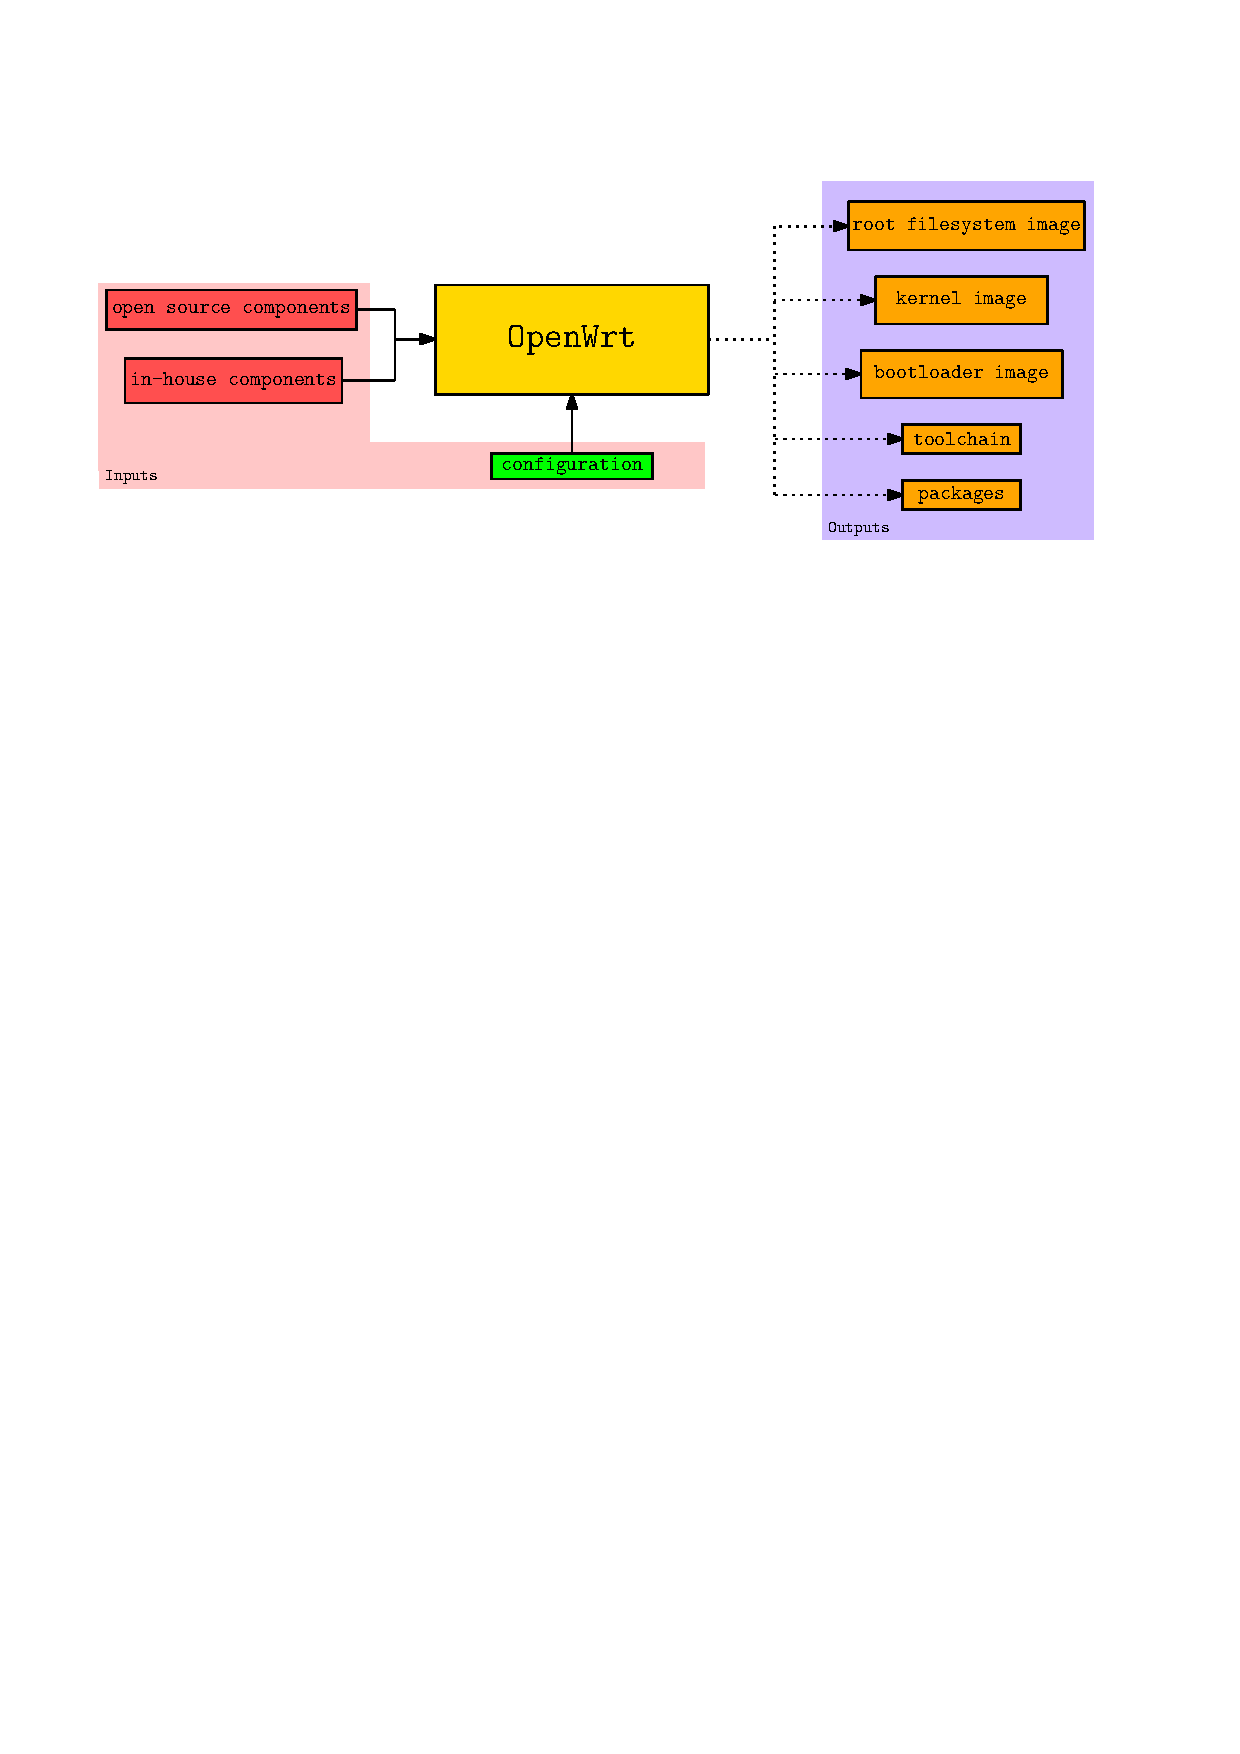
\includegraphics[width=1.5\textheight,keepaspectratio]{openwrt-composition}}
\end{frame}

\subsection{Build System}
\begin{frame}{Build System}
    \begin{itemize}[<+(1)->]
        \item Based on Buildroot~\cite{buildroot}.
        \item Automates process of porting software to specific hardware.
        \item Uses Kconfig~\cite{linux-kconfig} for configuration of features.
        \item Provides integrated cross-compiler toolchain.
        \item Provides abstraction for Autotools~\cite{gnu-autotools}, CMake~\cite{kitware-cmake}, SCons~\cite{scons}.
        \item Provides patch management with Quilt~\cite{fsf-quilt}.
        \item Provides download, patch, configure, compile and packaging workflow.
    \end{itemize}
\end{frame}

\section{Building and Running OpenWrt}

\subsection{Preparing Host}
\begin{frame}{Preparing Host}
    \begin{itemize}[<+(1)->]
        \item Build system works on Linux, BSD or macOS operating system. \textbf{Microsoft Windows is NOT supported.}
        \item Recommendation is to use Linux distribution, specifically Debian~\cite{debian-website}.
        \item \href{https://openwrt.org/docs/guide-developer/build-system/install-buildsystem}{Official} documentation describing OpenWrt build system requirements in details.
        \item Personal recommendation is to use a \href{https://github.com/hvarga/openwrt-application-development/blob/master/presentation/resources/Dockerfile}{custom made} Docker Image which includes everything necessary for building OpenWrt.
        \item Download OpenWrt project source code.
        \begin{itemize}
            \item \texttt{git clone https://git.openwrt.org/openwrt/openwrt.git}
        \end{itemize}
        \item Checkout latest stable version.
        \begin{itemize}
            \item \texttt{git checkout v17.01.4}
        \end{itemize}
    \end{itemize}
\end{frame}

\subsection{Configuring Build System}
\begin{frame}{Configuring Build System}
    \begin{itemize}[<+(1)->]
        \item Prepare package feed.
        \begin{itemize}
            \item \texttt{cp feeds.conf.default feeds.conf}
        \end{itemize}
        \item Update package index based on the information available in the feeds.
        \begin{itemize}
            \item \texttt{./scripts/feeds update -a}
        \end{itemize}
        \item Make all packages in feeds available in the configuration menu.
        \begin{itemize}
            \item \texttt{./scripts/feeds install -a}
        \end{itemize}
        \item Start the build system configuration interface and select target platform, packages to be compiled, packages to be included in the firmware file, kernel options, and much more.
        \begin{itemize}
            \item \texttt{make menuconfig}
        \end{itemize}
    \end{itemize}
\end{frame}

\begin{frame}{Configuring Build System}
    \centerline{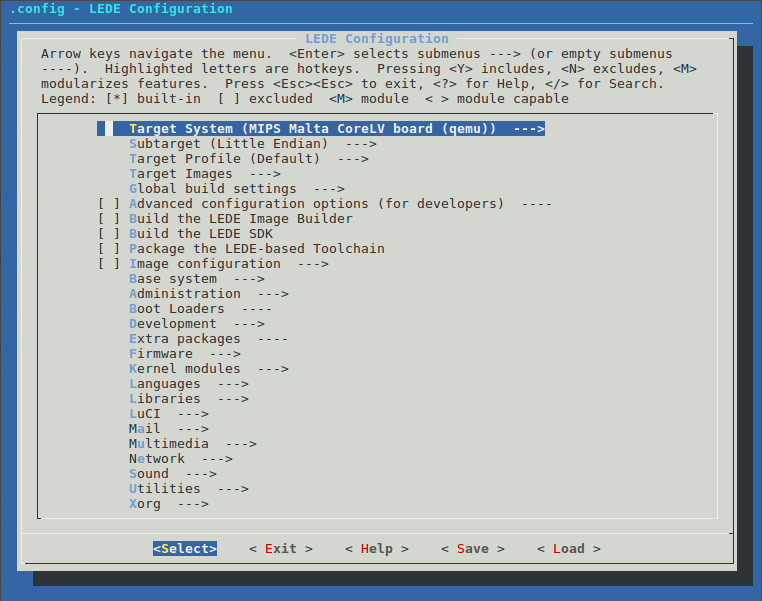
\includegraphics[height=0.8\textheight,keepaspectratio]{menuconfig}}
\end{frame}

\begin{frame}{Configuring Build System}
    %{\large Example of targets and its usage.}
    Example of targets and its usage
    \begin{itemize}[<+(1)->]
        \item Dedicated hardware. Example, choose \texttt{Broadcom BCM27xx} for Target System and \texttt{BCM2710} for Subtarget to configure build system for Raspberry Pi 3.
        \item Virtualized using QEMU. Example, choose \texttt{MIPS Malta CoreLV board (qemu)} for Target System to get a QEMU compatible image.
        \item Containerized environment using Docker. Example, choose \texttt{x86} for Target System to get an image which can be imported into Docker.
    \end{itemize}
\end{frame}

\subsection{Building and Running Image}
\begin{frame}{Building and Running Image}
    \begin{itemize}[<+(1)->]
        \item It is assumed that you have choosen \textit{MIPS Malta CoreLV board (qemu)} for Target System.
        \item Build the final image.
        \begin{itemize}
            \item \texttt{make}
        \end{itemize}
        \item Images can be found under the \texttt{./bin/targets/} directory. For \textit{MIPS Malta CoreLV board (qemu)}, images are stored in \texttt{.bin/targets/malta/le/}.
        \item Run the image in QEMU.
        \begin{itemize}
            \item \texttt{cd ./bin/targets/malta/le}
            \item \texttt{qemu-system-mipsel} \\
                  \texttt{-kernel lede-malta-le-vmlinux-initramfs.elf} \\
                  \texttt{-nographic}
        \end{itemize}
    \end{itemize}
\end{frame}